\section{Factorial Design}
\begin{frame}
  \begin{center}
    {\bf Part III - Factorial Design}
  \end{center}
\end{frame}

\begin{frame}{Factorial Designs}
  Many experiments involve more than one factor of interest. Sometimes we want
  to control {\bf multiple independent variables} that influence the response of the experiment.
  \bigskip

  One effective way to explore the main effects and interactions of multiple factors is
  the {\bf Factorial Design}. In a factorial design, all level combinations are
  explored.\vfill

  \begin{block}{Main Effect and Interaction}
    \begin{itemize}
      \item {\bf Main Effect} of a factor: The mean change of the response variable when we change the level of a factor;
      \bigskip

      \item {\bf Interaction} between factors: The mean change of the response variable when we change the level of two or more factors at the same time.
    \end{itemize}
  \end{block}
\end{frame}

\begin{frame}{Factorial Design Example}

  \begin{columns}
    \column{.1\textwidth}
    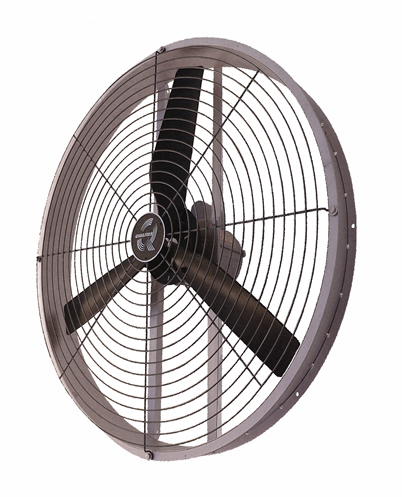
\includegraphics[width=1\textwidth]{../img/ventilador.png}
    \ppagenote{Ventilator figure from http://refrigelms.com.br}
    \column{.9\textwidth}
    An engineer wants to investigate factors that affect the electrical current demanded by a motor used in the ventilation of a chicken coop. She identifies two factors to investigate regarding the current demand of a motor:
  \end{columns}
  \begin{itemize}
    \item {\bf Factor 1:} The manufacturer of the motor (levels: A, B, C)
    \item {\bf Factor 2:} The state of the motor (levels: original, rewinded)
  \end{itemize}\bigskip

  To investigate this question, the engineers sample a 40 motors from each manufacturer, 20 in the original state, and 20 being rewinded motors. The current draw from each motor is registered. (See data file "motors.txt")
\end{frame}

\begin{frame}[fragile]{Example: Exploratory Data Analysis}

  {\smaller
\begin{verbatim}
> data <- read.table("../data files/motors.txt", header = TRUE)
> library(ggplot2)
> p <- ggplot(data, aes(x = Manufacturer, y = Current.Amperes,
                        fill = Manufacturer))
> p + geom_boxplot() + facet_grid(.~State) + ...
\end{verbatim}
  }

  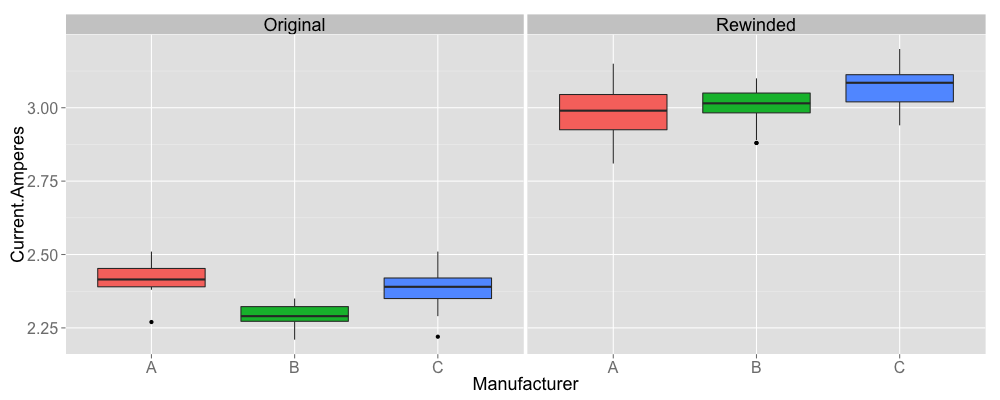
\includegraphics[width=.8\textwidth]{../img/motors_box1.png}
\end{frame}

\begin{frame}[fragile]{Example: Exploratory Data Analysis}

  The exploratory plot suggests a large main effect for the \emph{State} factor,
  and is inconclusive for the effect of the \emph{Manufacturer} factor. It is
  unclear if there are interaction effects or not.\bigskip

  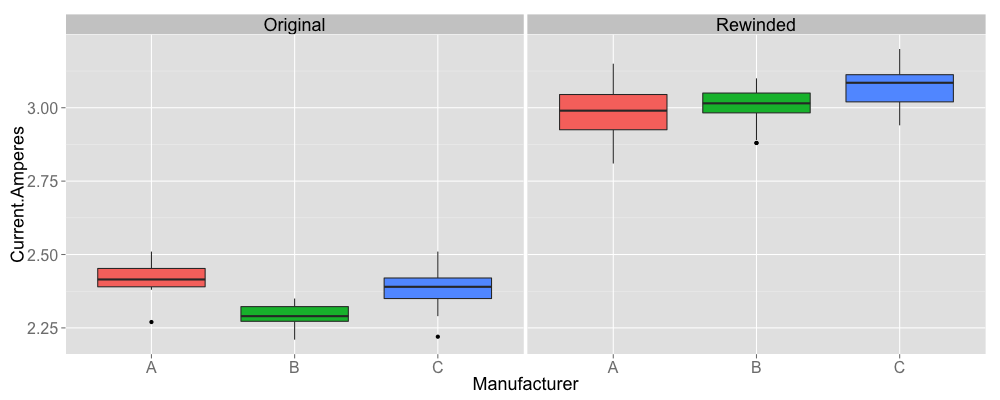
\includegraphics[width=.8\textwidth]{../img/motors_box1.png}
\end{frame}

\begin{frame}{Factorial Design Model}

  In the general case for a completely randomized factorial design we have:

\begin{itemize}
  \item \textit{a} levels for factor \textbf{A};
  \item \textit{b} levels for the factor \textbf{B};
  \item \textit{n} replicates within each combination of levels;
  \item Completely randomized collection of observations;
\end{itemize}\bigskip

  The {\bf additive effects model} for a set of observations collected following this design can be expressed as follows. From this model, we can construct null/alternate hypotheses in a similar fashion as in ANOVA.

  \begin{equation*}
  y_{ijk} = \mu+\tau_i+\beta_j+(\tau\beta)_{ij}+\epsilon_{ijk}\begin{cases}
  i=1,\ldots,a\\
  j=1,\ldots,b\\
  k=1,\ldots,n
\end{cases}\end{equation*}
\end{frame}

\begin{frame}[fragile]{Statistical Model for Two Factors}

The ANOVA gives us the linear model for the mean effect of each
factor (State, Manufacturer), as well as the interaction effect (State x Manufacturer).
\medskip

By analysing these effects, we can define our post-hoc analysis.

{\smaller
\begin{verbatim}
> model <- aov(Current.Amperes~State*Manufacturer,
+              data = data)
> summary(model)
                    Df Sum Sq Mean Sq F value   Pr(>F)
State                1 12.956  12.956 2798.41  < 2e-16 ***
Manufacturer         2  0.118   0.059   12.71 1.04e-05 ***
State:Manufacturer   2  0.114   0.057   12.27 1.49e-05 ***
Residuals          114  0.528   0.005
---

> summary.lm(model)$r.squared
[1] 0.9615174
\end{verbatim}}
\end{frame}

\begin{frame}[fragile]{Examining the Data Assumptions}

As usual, the assumptions can be verified by means of residual analysis, like in the one-way ANOVA (except for a little adjustment needed for the Fligner-Killeen test)

{\smaller
\begin{verbatim}
> shapiro.test(model$residuals)
W = 0.9857, p-value = 0.2392

> fligner.test(Current.Amperes ~ interaction(State, Manufacturer),
+              data = data)
med chi-squared = 10.1721, df = 5, p-value = 0.0705
\end{verbatim}}

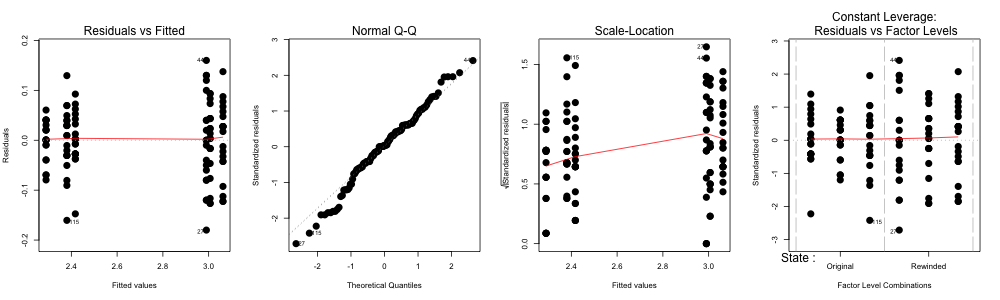
\includegraphics[width=.8\textwidth]{../img/motors_res.png}
\end{frame}

\begin{frame}{Factorial Design -- Post-hoc comparison}

If the ANOVA indicates the existence of significant effects, we can perform pairwise comparisons between levels to investigate specific differences;
\bigskip
When the interaction effect is not significant, the comparisons between factor levels can be done in a straightforward manner, using the estimated level means. For instance, the test statistic for comparing the means of levels 2 and 3 of factor A could be calculated as:

\begin{equation*}
t_0 = \frac{\bar{y}_{2\cdot\cdot} - \bar{y}_{3\cdot\cdot}}{\sqrt{2\frac{MS_E}{n'}}}
\end{equation*}

where $n'$ is the number of specific replicates for the comparison under consideration.
\end{frame}

\begin{frame}[fragile]{Factorial designs -- Post-hoc comparison}

More generally,
\begin{equation*}
t_0 = \frac{\Delta\bar{y}}{\sqrt{2\frac{MS_E}{n'}}}
\end{equation*}

For comparisons of factor levels (main effects), the value of $n'$ is the total number of observations under that level;
\bigskip

For comparisons of level combinations (interaction effects), it is the number of observations within each combination group;

\begin{verbatim}
> replications(Current ~ State*Manufacturer,
+              data = data)
             State       Manufacturer State:Manufacturer
                60                 40                 20
\end{verbatim}

Also, the $\alpha$ value for the comparisons has to be adjusted to prevent inflation of the type-I error rate.
\end{frame}






















%
